\documentclass[]{spie}  %>>> use for US letter paper
%\documentclass[a4paper]{spie}  %>>> use this instead for A4 paper
%\documentclass[nocompress]{spie}  %>>> to avoid compression of citations

\renewcommand{\baselinestretch}{1.0} % Change to 1.65 for double spacing
 
\usepackage{amsmath,amsfonts,amssymb}
\usepackage{graphicx}
\usepackage[colorlinks=true, allcolors=blue]{hyperref}


\usepackage{color}
\usepackage[latin9]{inputenc}
\usepackage{mathrsfs,amsmath}
\usepackage{graphicx}%
\usepackage{float}
\usepackage{amsfonts}%
\usepackage[titletoc]{appendix}
\usepackage{amssymb}
\usepackage{braket}
\usepackage{bm}

\newcommand{\mb}[1]{\bm{#1}}
\usepackage[T1]{fontenc}

\def\Nabla{\bm{\nabla}}
\def\bm{\mathbf}
\def\curl{\Nabla\times}
\def\div{\Nabla\cdot}
\def\lap{\Delta}
\def\vlap{\Delta}
\def\x{\hat{e}_{x}}
\def\y{\hat{e}_{y}}
\def\z{\hat{e}_{z}}
\def\p{\partial}
\def\h{\hat}
\def\h{\hat}
\def\tw{\tilde{\omega}}
\def\gm{\gamma}
\def\om{\omega}
\def\OM{\Omega}
\def\GM{\Gamma}
\def\dw{\delta\omega}
\def\dth{\Delta\theta}
\def\dk{\delta k}
\def\Hdth{\frac{\dth}{2}} %half Delta Theta


\title{Temporal Hole Burning in QCLs - derivation}


\author[a]{Petar Tzenov}
\date{June 6, 2016}%

\authorinfo{Further author information:\\a: E-mail: petar.tzenov@tum.de}

% Option to view page numbers
\pagestyle{empty} % change to \pagestyle{plain} for page numbers   
\setcounter{page}{301} % Set start page numbering at e.g. 301
 
\begin{document} 
\maketitle
 
 
 
\section{Equations of motion in the tight-binding approximation}

In the TB approximation the Hamiltonian matrix of a 3 level system with a single resonant tunneling and single optical transition, takes the form (in the rotating wave approximation)

\begin{align}
\label{eq:hamiltonian-matrixform}
H_{TB}^{RWA} &= \begin{pmatrix}
\hbar(\epsilon + \omega_{0} -\omega_c) & \hbar \Omega_{1'3} & 0 \\ 
\hbar \Omega_{1'3} & \hbar(\omega_{0} -\omega_c) & q_0d_{32}f/2 \\
0 & q_0d_{32}f^*/2 & 0
\end{pmatrix},
\end{align}
where $\hbar \Omega_{1'3}$ is 1/2 of the anti-crossing energy for the tunneling coupling between injector ($\ket{1'}$) and upper laser level ($\ket{3}$), $\hbar\epsilon = E_{1'}-E_{3}$ is the detuning from tunneling resonance, $f(x,t)$ denotes the complex electric field envelope, $\hbar\omega_{0}$ is the transition energy between the upper laser level ($\ket{3}$) and the lower laser level ($\ket{2}$), $d_{32} = \bra{3}\h{z}\ket{2}$ is the dipole matrix element, $q_0$ is the elementary charge, $\omega_0$ the field's carrier frequency. Expanding von Neumann's equation and including scattering terms (within the usual approach), we obtain the following system (for a ring cavity laser)
\begin{subequations}
	\label{eq:threelevelmodel}
	\begin{align}
	\frac{n}{c}\partial_t f &+ \partial_{x}f= -i\frac{N \Gamma q_0d_{32} k_c}{\epsilon_0 n^2} \eta_{32} - \frac{l_0}{2} f \label{eq:rtwave} \\
	\frac{d \rho_{1'1'}}{d t} 	&= i\Omega_{1'3} (\rho_{1'3} - \rho_{31'})+ \Gamma_{31'}\rho_{33} + \Gamma_{21'}\rho_{22}  -\Gamma_{1'}\rho_{1'1'} \\
	\frac{d \rho_{33}}{d t}	& = i\Omega_{1'3} (\rho_{31'} - \rho_{1'3}) + i\frac{q_0d_{32}}{2\hbar} \big (f^*\eta_{32}- c.c. \big ) 
	+\Gamma_{1'3}\rho_{1'1'} + \Gamma_{23}\rho_{22} - \Gamma_3 \rho_{33},  \\
	\frac{d \rho_{22}}{d t}  &= -i\frac{q_0d_{32}}{2\hbar} \big (f^*\eta_{32} - c.c. \big )  + \Gamma_{1'2}\rho_{1'1'}  +  \Gamma_{32}\rho_{33} - \Gamma_{2}\rho_{22} , \\
	\frac{d \rho_{1'3}}{d t}  &= -i\epsilon\rho_{1'3} +i \Omega_{1'3}(\rho_{1'1'} - \rho_{33}) +i\frac{q_0d_{32}}{2 \hbar}f^*\eta_{1'2}- \Gamma_{\parallel 1'3} \rho_{1'3},  \\
	\frac{d \eta_{32}}{d t}   &= i(\omega_c - \omega_0)\eta_{32} + i \frac{q_0d_{32}}{2\hbar}f(\rho_{33}-\rho_{22})  - i\Omega_{1'3}\eta_{1'2} - \Gamma_{\parallel 32}\eta_{32}, \\
	\frac{d \eta_{1'2}}{d t} &= i(\omega_c - \omega_0-\epsilon)\eta_{1'2} +i \frac{q_0d_{32}}{2\hbar}f\rho_{1'3} - i\Omega_{1'3}\eta_{32} - \Gamma_{\parallel 1'2}\eta_{1'2}.
	\end{align}
\end{subequations}

Let us further investigate the effect of the spectral splitting onto the temporal dynamics of our system by taking the following, additional ansatz for the envelope $f(x,t)$ and accordingly the coherences
\begin{subequations}
	\begin{align}
	\label{eq:splittingAnsatz}
	f &= f^{(\delta)}e^{ i(\dk x -\dw t)} + f^{(-\delta)}e^{-i(\dk x -\dw t)}, \\
	\eta_{32} &= \eta_{32}^{(\delta)}e^{i(\dk x -\dw t)} + \eta_{32}^{(-\delta)}e^{-i(\dk x -\dw t)}, \\
	\eta_{1'2} &= \eta_{1'2}^{(\delta)}e^{i(\dk x -\dw t)} + \eta_{1'2}^{(-\delta)}e^{-i(\dk x -\dw t)},
	\end{align}
\end{subequations}
where $\delta\omega$ is $\approx \Omega_{1'3}$ half of the anticrossing frequency of the tunneling transition. Next we use the above ansatz to evaluate the products $f^*\eta_{1'2}$ and $f^*\eta_{32}$ in Eq. (\ref{eq:threelevelmodel}). Using the index $j$ as a place holder for $1'2$ and  $32$ we obtain (assuming for simplicity that $x = 0$)

\begin{align}
\label{eq:feta-product}
f^{*}\eta_{j} &= ((f^{(\delta)})^*e^{  i\delta\omega t} + (f^{(-\delta)})^*e^{-i\delta\omega t})(\eta_{j}^{(\delta)}e^{ - i\delta\omega t} + \eta_{j}^{(-\delta)}e^{+i\delta\omega t}) \nonumber \\
&= \big[ (f^{(\delta)})^*\eta_{j}^{(\delta)} +(f^{(-\delta)})^*\eta_{j}^{(-\delta)} + (f^{(\delta)})^*\eta_{j}^{(-\delta)}e^{2i\delta\omega t} + (f^{(-\delta)})^*\eta_{j}^{(\delta)}e^{-2i\delta\omega t}\big ].
\end{align} 
We can reconcile this result with Eq. (\ref{eq:threelevelmodel}) if we extend it with the following ansatz for the  population densities and the $\rho_{1'3}$ coherence term 
\begin{align}
\rho_{jj} &= \rho_{jj}^{DC}+\rho_{jj}^{+}e^{2i(\dk x -\dw t)} + \rho_{jj}^{-}e^{-2i(\dk x -\dw t)}, \\
\rho_{1'3} &= \rho_{1'3}^{DC}+\rho_{1'3}^{+}e^{2i(\dk x -\dw t)} + \rho_{1'3}^{-}e^{-2i(\dk x -\dw t)},
\end{align}
where $j \in \{1',3,2\}$, $\rho_{jj}^{-} = (\rho_{jj}^{(+)})^*$ and $\rho_{1'3}^{-} = (\rho_{1'3}^{+})^*$ due to the Hermitian property of the density matrix. Then, we can derive the evolution equations for $\rho_{jj}^{DC},\rho_{jj}^{\pm}$ and $\rho_{1'3}^{DC},\rho_{1'3}^{\pm}$ as follows
\begin{subequations}
	\label{eq:mainsystem}
	\begin{align}
	\label{eq:temporal-hole-11}
	\frac{d\rho_{1'1'}^{DC}}{dt} &= i\Omega_{1'3}(\rho_{1'3}^{DC}-(\rho_{1'3}^{DC})^*) +  \Gamma_{31'}\rho_{33}^{DC} + \Gamma_{21'}\rho_{22}^{DC}  -\Gamma_{1'}\rho_{1'1'}^{DC}, \\
	\frac{d\rho_{1'1'}^{+}}{dt} &= 2i\delta\omega\rho_{1'1'}^{+} + i\Omega_{1'3}(\rho_{1'3}^{+}-(\rho_{1'3}^{-})^*) +  \Gamma_{31'}\rho_{33}^{+} + \Gamma_{21'}\rho_{22}^{+}  -\Gamma_{1'}\rho_{1'1'}^{+}, \\
	\label{eq:temporal-hole-33}
	\frac{d\rho_{33}^{DC}}{dt} &= -i\Omega_{1'3}(\rho_{1'3}^{DC}-(\rho_{1'3}^{DC})) + i\frac{q_0d_{32}}{2\hbar} \left [ ( f^{(\delta)})^*\eta_{32}^{(\delta)} +(f^{(-\delta)})^*\eta_{32}^{(-\delta)} -c.c.\right]
	+\Gamma_{1'3}\rho_{1'1'}^{DC} + \Gamma_{23}\rho_{22}^{DC} - \Gamma_3 \rho_{33}^{DC}, \\
	\frac{d\rho_{33}^{+}}{dt} &= 2i\delta\omega\rho_{33}^{+} - i\Omega_{1'3}(\rho_{1'3}^{+}-(\rho_{1'3}^{-})^*) + i\frac{q_0d_{32}}{2\hbar} \left [ (f^{(-\delta)})^*\eta_{32}^{(\delta)} -f^{(\delta)}(\eta_{32}^{(-\delta)})^*\right]
	+\Gamma_{1'3}\rho_{1'1'}^{+} + \Gamma_{23}\rho_{22}^{+} - \Gamma_3 \rho_{33}^{+}, \\
	\frac{d\rho_{22}^{DC}}{dt} &= -i\frac{q_0d_{32}}{2\hbar} \left [ ( f^{(\delta)})^*\eta_{32}^{(\delta)} +(f^{(-\delta)})^*\eta_{32}^{(-\delta)} -c.c.\right]
	+\Gamma_{1'2}\rho_{1'1'}^{DC} + \Gamma_{32}\rho_{33}^{DC} - \Gamma_2 \rho_{22}^{DC}, \\
	\frac{d\rho_{22}^{+}}{dt} &= 2i\delta\omega\rho_{22}^{+} - i\frac{q_0d_{32}}{2\hbar} \left [ (f^{(-\delta)})^*\eta_{32}^{(\delta)} -f^{(\delta)}(\eta_{32}^{(-\delta)})^*\right]
	+\Gamma_{1'2}\rho_{1'1'}^{+} + \Gamma_{32}\rho_{33}^{+} - \Gamma_2 \rho_{22}^{+}, \\
	\frac{d \rho_{1'3}^{DC}}{d t}  &= -i\epsilon\rho_{1'3}^{DC} +i \Omega_{1'3}(\rho_{1'1'}^{DC} - \rho_{33}^{DC}) +i\frac{q_0d_{32}}{2 \hbar}((f^{(\delta)})^*\eta_{1'2}^{(\delta)} +(f^{(-\delta)})^*\eta_{1'2}^{(-\delta)})
	-\Gamma_{\parallel 1'3} \rho_{1'3}^{DC},  \\
	\frac{d \rho_{1'3}^{\pm}}{d t}  &= -i(\epsilon \mp 2\delta\omega)\rho_{1'3}^{\pm} +i \Omega_{1'3}(\rho_{1'1'}^{\pm} - \rho_{33}^{\pm}) +i\frac{q_0d_{32}}{2 \hbar}( (f^{(\mp\delta)})^*\eta_{1'2}^{(\pm\delta)} )- \Gamma_{\parallel 1'3} \rho_{1'3}^{\pm},\\
	\frac{d \eta_{32}^{(\pm\delta)}}{d t} &= -i(\Delta \mp \delta\omega)\eta_{32}^{(\pm\delta)}
	+i\frac{q_0d_{32}}{2\hbar} \left[ f^{(\pm\delta)}(\rho_{33}-\rho_{22})^{DC} + f^{(\mp \delta)} (\rho_{33}^{\pm}-\rho_{22}^{\pm})\right]-i\Omega_{1'3}\eta_{1'2}^{(\pm\delta)}- \Gamma_{\parallel 32}\eta_{32}^{(\pm\delta)}, \label{eq:eta_1'3-temphole} \\
	\frac{d \eta_{1'2}^{(\pm\delta)}}{d t} &= -i(\Delta+\epsilon \mp \delta\omega)\eta_{1'2}^{(\pm\delta)}+i\frac{q_0d_{32}}{2\hbar} ( f^{(\pm\delta)}\rho_{1'3}^{DC} + f^{(\mp \delta)} \rho_{1'3}^{\pm})-i\Omega_{1'3}\eta_{32}^{(\pm\delta)}-
	\Gamma_{\parallel 1'2}\eta_{1'2}^{(\pm\delta)}, \label{eq:eta_1'2-temphole}
	\end{align} 
\end{subequations}
where $\Delta = \omega_0 - \omega_c$ denotes the detuning of the carrier frequency from $3\leftrightarrow2$ resonance. 

The coefficients $\Gamma_{ij} $ are the scattering rates from state $\ket{i}$ to state $\ket{j}$, $\Gamma_k = \sum_{j}\Gamma_{kj}$ is the total out-scattering rate from level $\ket{k}$ and $\Gamma_{\parallel ij} = \frac{1}{2}(\Gamma_{i} + \Gamma_j) + \Gamma_{i,j}^*$ with $\Gamma_{i,j}^*$ the pure dephasing rate for the transition $i\rightarrow j$ and we have include a linear power loss term $l_0$ in the envelope propagation equations. 

It is worthwhile to notice, however, that in the derivation of the time evolution equations for $\eta_{1'2}^{\pm\delta}$ and $\eta_{32}^{\pm\delta}$, we have omitted terms proportional to $f^{\pm\delta}\rho_{1'3}^{\pm}exp\{\pm3i(\dk x - \dw t)\}$ and $f^{\pm\delta}(\rho_{33}^{\pm}-\rho_{22}^{\pm})exp\{\pm3i(\dk x - \dw t)\}$, respectively, which is to say that we neglect scattering of $f^{\pm\delta}$ off the corresponding parts of the grating.

The field components evolve according to
\begin{align}
\frac{n}{c}\partial_t f^{(\pm \delta)} + \partial_{x}f^{(\pm \delta)}&= -i\frac{N \Gamma q_0d_{32} k_c}{\epsilon_0 n^2} \eta_{32}^{(\pm \delta)}  \nonumber \\ 
&-\left[\frac{l_0}{2}  \mp i (\frac{n\delta\omega}{c}-\delta k)\right] f^{(\pm \delta)}\label{eq:rtwave-temphole}.
\end{align}


\section{Density matrix equations in the dressed states basis}
\label{sec:biasdependence}
 
 The introduction of the coupling energy $\hbar \Omega_{1'3}$ into the Hamiltonian of the system contributes to a splitting of the optical spectra into a high and a low frequency lobes. This is due to the fact that the original system's Hamiltonian is non-diagonal in the tight binding basis. The new eigenstates, which in the absence of electromagnetic radiation, i.e. $f(x,t) \approx 0$, diagonalize the Hamiltonian in Eq. (\ref{eq:hamiltonian-operatorform}), are the so called delocalized, or dressed, states and are obtained from the tunneling levels $\Ket{1'}$ and $\Ket{3}$ via the unitary transformation
 \begin{align}
 \label{eq:dressedstates}
 \Ket{+} &= \cos\theta \Ket{1'} - \sin\theta \Ket{3}, \nonumber \\
 \Ket{-} &= \sin\theta \Ket{1'} + \cos\theta \Ket{3}.
 \end{align}
 The corresponding energies are given by $E_\pm =\hbar(\omega_0 +\epsilon/2) \pm \hbar \left(\epsilon^2+4\Omega_{1'3}^2\right )^{1/2}$, and the expansion coefficients are computed from   
 $
 \tan \theta = -2\Omega_{1'3}/[\epsilon+(\epsilon^2+4\Omega_{1'3}^2)^{1/2}].
 $
 Within the full extended basis picture, where the wave functions are calculated for several neighbouring periods, these tight-binding states are simply split electron states spanning the intermodule barrier, see Fig. \ref{fig:basis_schemata}b. Both dressed states  couple radiatively to the lower laser level $\ket{2}$, since they both have a component in the $\ket{3}$ direction in the tight binding expansion. We can calculate the ratio of the dipole matrix elements for the $\Ket{+}\leftrightarrow\Ket{2}$ and $\Ket{-}\leftrightarrow\Ket{2}$ transitions, which will determine the relative strength between the high and low frequency lobes of the gain. If we assume that the $d_{1'2} \approx 0$, which is reasonable in the tight binding basis due to the negligible overlap between wave function in different modules, we obtain  $|\Bra{+}\hat{z}\Ket{2}|/|\Bra{-}\hat{z}\Ket{2} | \approx |\tan\theta| =  2|\Omega_{1'3}|/|\epsilon+\sqrt{\epsilon^2+4\Omega_{1'3}^2}|$. We now can see that at positive detunings $\epsilon >0$, $|\tan\theta|<1$ and thus the low frequency transition will have higher probability. On the other hand, for $\epsilon < 0 $ we get that $|\tan\theta| >1$ which will lead to lasing predominantly in the high frequency regime.

\begin{figure}[h!]
	\begin{center}
		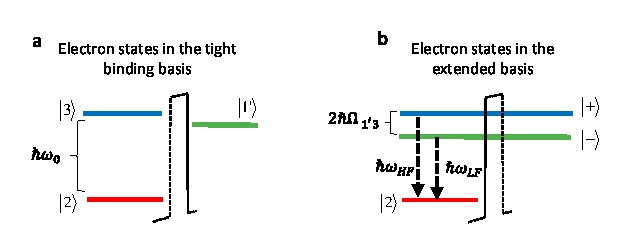
\includegraphics[scale=1]{BASISPICTURE.eps}
		\caption{ Schematic illustration of the tight binding \textbf{a} and extended basis \textbf{b}, states.  } \label{fig:basis_schemata}
	\end{center}	
\end{figure}
\section{Extended basis EOM}
Within the delocalized basis picture the observed pulse switching behaviour has a very intuitive and simple explanation. If we apply the unitary transform given by Eq. (\ref{eq:dressedstates}) onto the tight binding Hamiltonian and also employ the rotating wave approximation, the Hamiltonian and the statistical operator can be cast in the following matrix form
\begin{equation}
H^{\text{RWA}} = \begin{bmatrix}
\hbar (\omega_+-\omega_c) & 0 & q_0d_{+2}f/2 \\
0 & \hbar (\omega_--\omega_c) & q_0d_{-2}f/2 \\
q_0d_{+2}f^*/2 & q_0d_{-2}f^*/2 & 0 \\
\end{bmatrix},\quad \rho^{\text{RWA}} = \begin{pmatrix}
\rho_{++} & \rho_{+-} & \eta_{+2} \\ 
\rho_{-+} & \rho_{--} & \eta_{-2} \\ 
\eta_{2+} & \eta_{2-} & \rho_{22} \\ 
\end{pmatrix}.
\end{equation}
The symbols $d_{+2} = \Bra{+}\hat{z}\Ket{2} $ and $d_{-2} = \Bra{-}\hat{z}\Ket{2} $, denote the corresponding dipole moments, and $ \eta_{\pm 2}$ the slowly varying coherences. 

In this basis, the von Neumann equation reads (neglecting collision terms)
\begin{subequations}
\begin{align}
\frac{d \rho_{++}}{dt} &= i\frac{q_0d_{+2}}{2\hbar}(f^*\eta_{+2}-f\eta_{+2}^*), \\
\frac{d \rho_{--}}{dt} &= i\frac{q_0d_{-2}}{2\hbar}(f^*\eta_{-2}-f\eta_{-2}^*), \\
\frac{d \rho_{22}}{dt} &= -i\frac{q_0d_{+2}}{2\hbar}(f^*\eta_{+2}-f\eta_{+2}^*)-i\frac{q_0d_{-2}}{2\hbar}(f^*\eta_{-2}-f\eta_{-2}^*), \\
\frac{d \rho_{+-}}{dt} &= -i(\omega_+-\omega_-)\rho_{+-}-i\frac{q_0d_{+2}}{2\hbar}f\eta_{2-}+i\frac{q_0d_{-2}}{2\hbar}f^*\eta_{+3},\\
\frac{d \eta_{+2}}{dt} &= -i(\omega_+-\omega_0)\eta_{+2}+i\frac{q_0d_{+2}}{2\hbar}f(\rho_{++}-\rho_{22})+i\frac{q_0d_{-2}}{2\hbar}f\rho_{+-}, \label{eq:eta+2}\\
\frac{d \eta_{-2}}{dt} &= -i(\omega_--\omega_0)\eta_{-2}+i\frac{q_0d_{-2}}{2\hbar}f(\rho_{--}-\rho_{22})+i\frac{q_0d_{+2}}{2\hbar}f\rho_{-+}. \label{eq:eta-2}
\end{align}
\end{subequations}
Now, if we assume that $f = f^*$,  $\epsilon \approx 0$ and also that $d_{+2}\approx d_{-2} = d$, it turns out that we can reduce the $3-$level delocalized state system into a quasi-2-level system, by setting  $\eta = \eta_{+2}+(\eta_{-2})^*$ and deriving the time evolution of this quantity. Adding Eq. (\ref{eq:eta+2}) with the complex conjugate of Eq. (\ref{eq:eta-2}), we obtain
\begin{equation}
\label{eq:coherence_quasi2lvl}
\frac{d \eta}{dt} = -2i\Omega_{1'3} \eta + i\frac{q_0d}{2\hbar}fw, 
\end{equation}
where $w = \rho_{++}-\rho_{--}$ denotes the inversion between the delocalized states, which	 evolves according to 
\begin{align}
\label{eq:inversion_quasi2lvl}
\frac{d w }{dt}	&=  i\frac{q_0d}{2\hbar}f(\eta-\eta^*).
\end{align}
We thus see that under the above idealized assumptions, we have reduced the three level system into an effective two level such. In fact, this is a "quasi" two level system due to the presence of a factor of 2 in the denominator of Eq. (\ref{eq:inversion_quasi2lvl}), which distinguishes it from the standard Bloch equations \cite{boyd2003nonlinear}.

To see why Eqs. (\ref{eq:coherence_quasi2lvl}) and (\ref{eq:inversion_quasi2lvl}) could lead to a pulse switching behaviour we need to include the optical field propagation equations into the model. For classical fields, absence of free electric charges and weak inhomogeneities, the electric field envelope (within the slowly varying amplitude approximation) obeys the propagation equation
\begin{align}
	\frac{n_0}{c} \p_t f - \p_x f = -i\frac{N \Gamma q_0d k_c}{\epsilon_0 n^2}(\eta_{+2}+\eta_{-2}),
\end{align}
where $\epsilon_0$ is the permittivity of free space and $N$ is the average carrier density per unit volume. Now decomposing the polarization envelopes, $\eta_{+2}$ and $\eta_{-2}$ into their real and imaginary parts, i.e. $\eta_{+2} = u_{+}+iv_{+}$ and $\eta_{-2} = u_{-}+iv_{-}$, and plugging into the propagation equation we obtain that
\begin{align}
\label{eq:field_propagation}
\frac{n}{c} \p_t f - \p_x f = -i\frac{N \Gamma q_0d k_c}{\epsilon_0 n^2}(u_{+}+u{-}) + \frac{N \Gamma q_0d k_c}{\epsilon_0 n^2}(v_{+}+v_{-}).
\end{align}
The right hand side of Eq. (\ref{eq:field_propagation}) has straightforward interpretation. While the real part of the polarization is proportional to the change in the real part of the refractive index, the imaginary parts capture the electric field loss/gain due to the resonant transition. On the other hand, from the quasi two level system Eq. (\ref{eq:inversion_quasi2lvl}), we see that the \emph{difference} of the imaginary parts of the coherences, i.e. $v_{+}-v_{-} = \Im\{\eta\}$, has the same time evolution. This means that the high frequency transition's gain ($\ket{+}\leftrightarrow\ket{2}$) and low frequency transition's ($\ket{-}\leftrightarrow\ket{2}$) loss form a co-propagating quasi particle and vice versa. This intuitively explains how the coherent time evolution of the quasi-two level system would lead to a pulse switching behaviour, which has already been observed by experiment\cite{burghoff2015evaluating} and also captured by our simulations.
 
Lastly, we will elaborate a little further in order to reveal the time evolution of this quasi two level system by casting it into Bloch form. The standard substitutions, $u=(\eta + \eta^*)/2$, $v = -i(\eta - \eta^*)/2$ and as before $w = \rho_{++}-\rho_{--}$, in Eq. (\ref{eq:inversion_quasi2lvl}) and (\ref{eq:coherence_quasi2lvl}), yield what we will call the "quasi-Bloch equations"
\begin{subequations}
\label{eq:quasi-Blocheqn}
\begin{align}
\dot{u} &= 2\Omega_{1'3} v - \frac{u}{T_2}, \\
\dot{v} &= -2\Omega_{1'3} u +\beta w - \frac{v}{T_2}, \\
\dot{w} &= -2\beta v - \frac{w-w^0}{T_1},
\end{align}
\end{subequations}
where $\beta(t) = f(t)q_0d/2\hbar$ is the Rabi frequency. In Eq. (\ref{eq:quasi-Blocheqn}) we have also phenomenologically included effective dephasing times $T_1$ and $T_2$ as well as the steady state value of the inversion $w^0$. Notice that the above are \emph{not} the familiar Bloch equations due to the presence of a factor of $2$ in the equation for $\dot{v}$ and therefore the solutions (in the fully coherent case) do \emph{not} lie on the Bloch sphere of radius 1. When we neglect dephasing, we can see that $d(u^2+v^2+w^2)/dt = -2\beta vw \neq 0$ is actually not a conserved quantity. Analytical solution of the quasi-Bloch system are out of the scope of this work, however we present numerical such in the case of infinitely large coherence times. Solving Eq. (\ref{eq:quasi-Blocheqn}) reveals that the system dynamics is governed by two time scales, one fast oscillating term with a period 
close to $1/(2\Omega_{1'3}$, which is driven by the beating between the high and low frequency lobes, and another, slower time-scale the period of which is seen to increase with the maximum magnitude of the Rabi frequency $\beta(t)$. If we simply assume that $\beta(t) = \beta_0 \cos\omega_f t$, where $\omega_f$ is t, we find fact, the system in Eq. (\ref{eq:quasi-Blocheqn}) exhibits strong resonance at $\omega_f = 2\Omega_{1'3}$. To illustrate that, Fig. \ref{fig:quasi-bloch-off-resonance} displays the numerical solution of the quasi-Bloch equations, in the case when  $\omega_f = 1.9\Omega_{1'3}$, whereas Fig. \ref{fig:quasi-bloch-resonance} when $\omega_f = 2\Omega_{1'3}$.


\begin{figure}[h!]
	\begin{center}
		\includegraphics[scale=1]{quasi-bloch-off-resonance.eps}
		\caption{ Put Caption Here } \label{fig:quasi-bloch-off-resonance}
	\end{center}	
\end{figure}


\begin{figure}[h!]
	\begin{center}
		\includegraphics[scale=1]{quasi-bloch-resonance.eps}
		\caption{ Put Caption Here } \label{fig:quasi-bloch-resonance}
	\end{center}	
\end{figure}



\begin{figure}[h!]
	\begin{center}
		\includegraphics[scale=.25]{spheres.eps}
		\caption{ Put Caption Here } \label{fig:spheres}
	\end{center}	
\end{figure}


A few comments on the assumptions made in the above derivations are in order. First of all, it will be interesting to consider when will the reality condition for the envelope $f(x,t) $  hold. To investigate that, let us take an input pulse $f_{in}(t_0) = f(x=0,t_0)$, with Fourier transform $F_{in}(\omega)$, entering the medium at the left facet, such that at $F_{in}(\omega)^* = F_{in}(-\omega)$, i.e. $f_{in}$ is real. After propagating a distance $L$ inside the cavity the pulse transforms according to \cite{weiner2011ultrafast}
\begin{align}
\label{eq:fout-expansion}
f(x=L,t) &= \int_{-\infty}^{\infty} F(x=L,\omega)e^{-i\omega t}d\omega = \int_{-\infty}^{\infty} F_{in}(\omega)e^{-i\omega t}e^{g(\omega)L+i\Psi(\omega)}d\omega,
\end{align}
where $g(\omega)$ denotes the spectral gain per unit length and $\Psi(\omega)=k(\omega)L$, the acquired phase. In order for $f(x=L,t)$ to remain real, it is sufficient that $F(x=L,\omega)^*= F(x=L,-\omega)$. To find when this holds, we first expand the wave number $k(\omega)$ around $\omega=0$ up to fourth order to get  
\begin{align}
\label{eq:k-expansion}
k(\omega) = \beta_1\omega + \frac{\beta_2}{2}\omega^2 + \frac{\beta_3}{6}\omega^3 + O(\omega^4), 
\end{align}
which is justified since, by virtue of the rotating wave approximation, we had centred the spectrum around zero and also subtracted out $\beta_0 = k_c$ as the wave number at the central frequency $\omega_c$. Now from Eqs. (\ref{eq:fout-expansion}) and (\ref{eq:k-expansion}), we can write (neglecting terms $\propto O(\omega^4)$)
\begin{subequations}
	\begin{align}
		F(x=L,\omega)^* &\approx F_{in}(\omega)^* \exp\{g(\omega)L-i(\beta_1\omega + \frac{\beta_2}{2}\omega^2 + \frac{\beta_3}{6}\omega^3 )L\}, \\
		F(x=L,-\omega) &\approx F_{in}(-\omega) \exp\{g(-\omega)L+i(-\beta_1\omega + \frac{\beta_2}{2}\omega^2 - \frac{\beta_3}{6}\omega^3 )L\},
	\end{align}
\end{subequations}
which will be equal if
\begin{subequations}
	\begin{align}
	g(-\omega) &= g(\omega), \label{eq:symmetric-gain}\\
	\beta_2 = \beta_4 &= ... = \beta_{2n}=0. \label{eq:vanish-even-order-dispersion}
	\end{align}
\end{subequations}
The symmetric gain condition, Eq. (\ref{eq:symmetric-gain}), will be satisfied when the device is biased at injector $\leftrightarrow$ upper laser level resonance, as elaborated in Sec. \ref{sec:biasdependence}. On the other hand Eq. (\ref{eq:vanish-even-order-dispersion}) requires vanishing even order dispersion. We note that the comb in Ref. \cite{burghoff2014terahertz} probably approximately satisfies this condition, due to the incorporation of a dispersion compensation mechanism designed specifically to cancel the GVD coefficient $\beta_2$.

Lastly, the second assumption we made was that the dipole moments have equal algebraic value, i.e. $d_{+2} = d_{-2} = d$. What if they have opposite signs, i.e. $d_{+2} = -d_{-2} = d$? It is very easy to show that one can derive an equivalent quasi-two level system, but this time with the coherence set as $\eta = \eta_{+2}-\eta_{-2}^*$, instead of the substitution made above. In this case, the interpretation of the pulse switching behaviour remains the same, as the reader can readily verify by him/her-self.
\acknowledgments % equivalent to \section*{ACKNOWLEDGMENTS}       

% References
\bibliographystyle{spiebib}
\bibliography{../../literature/bib_resources}


\end{document} 
